\normaltrue \difficilefalse \tdifficilefalse
\correctionfalse
%\UPSTIidClasse{11} % 11 sup, 12 spé
%\newcommand{\UPSTIidClasse}{11}

\exer{Exercice EPAS $\star$ \label{PERF:02:C2:03:stab:64}}
%% CCP MP 2007
\setcounter{question}{0}\marginnote{\xpComp{PERF}{02}}%\index{Compétence C2-03}\index{Compétence PERF-02}
\index{Compétence C2-03}
\index{Schéma-blocs}
\index{Stabilite}

\ifcorrection
\else
\marginnote{\textbf{Pas de corrigé pour cet exercice.}}
\fi


\ifprof
\else
L'asservissement est donné par le schéma-blocs suivant. $H_{\text{BO}}(p) = \dfrac{4}{p\left( p+3,6\right)}$.  Le retard du système est de \SI{0,2}{s}.
De plus, $C(p)=K_c\dfrac{1+T_c p}{T_c p}$

\begin{marginfigure}
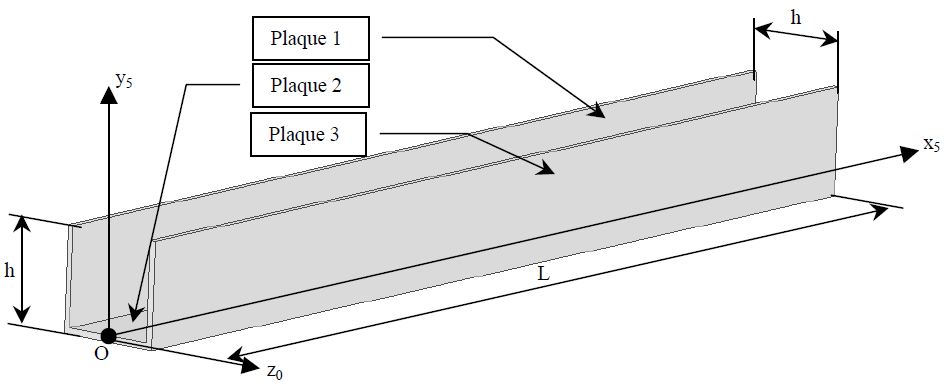
\includegraphics[width=\linewidth]{64_01}
\end{marginfigure}

\fi
 
\question{Tracer le diagramme de Bode asymptotique de $H_{\text{BO}}(p)$ pour des pulsations comprises entre \SI{0,5}{rad.s^{-1}} et \SI{50}{rad.s^{-1}}.}
\ifprof

\begin{figure}[!h]
 \begin{tikzpicture}[xscale=2]
\tikzset{
semilog lines/.style={thin, bleuxp}, 
semilog lines 2/.style={semilog lines,bleuxpc},
semilog half lines/.style={semilog lines 2,dotted },
semilog label x/.style={semilog lines,below,font=\tiny,black},
semilog label y/.style={semilog lines,right,font=\tiny,black}
}
\begin{scope}[yscale=1/60]
\OrdBode{20}
\semilog{-1}{2}{-80}{40}

\BodeAmp[bleuxp,thick]{-1:2}{\POAmpAsymp{1}{3.6}+\IntAmp{4}}
\BodeAmp[orangexp,ultra thick]{-1:2}{\POAmp{1}{3.6}+\IntAmp{4}}
%\draw (-2.2,27) node {\footnotesize 23,5 dB, 0 dB/d\'ecade};
%\draw (-3.5,120) node {\footnotesize $-$20 dB/d\'ecade};
%\draw (-1.5,65) node {\footnotesize $-$40 dB/d\'ecade};
%\draw [dashed,ultra thick,bleuxp] (-2.47,-1) -- (-2.47,80);
%\draw (-2.47,-1)  node {\Huge $\cdot$} node [above right]{\footnotesize $\dfrac{1}{300}$};
\end{scope}
\begin{scope}[yshift=-2cm,yscale=1/150]
\UniteDegre
\OrdBode{45}
\semilog{-1}{2}{-270}{0}
%\BodeArg[orangexp,samples=200,thick]{-1:1}{\POArgAsymp{40.}{300.}+\IntArg{1}}
\BodeArg[bleuxp,thick]{-1:2}{\POArgAsymp{4}{3.6}+\IntArg{1}}
\BodeArg[orangexp,ultra thick]{-1:2}{\POArg{4}{3.6}+\IntArg{1}}
\end{scope}
\end{tikzpicture}
\end{figure}
\else 
\fi

\question{Tracer le diagramme de Bode du retard pour des pulsations comprises entre \SI{0,5}{rad.s^{-1}} et \SI{50}{rad.s^{-1}}.}

\ifprof
Quelle que soit la valeur du retard, il n'a aucune influence sur le gain. La phase du retard est de $-0,2\omega$ soit $-\SI{0,2}{rad} = -11\degres$ en $\omega = \SI{1}{rad/s}$ et $-\SI{2}{rad} = -114\degres$ en $\omega = \SI{10}{rad/s}$.

\marginnote{Mauvais tracé...}
\begin{figure}[!h]
 \begin{tikzpicture}[xscale=2]
\tikzset{
semilog lines/.style={thin, bleuxp}, 
semilog lines 2/.style={semilog lines,bleuxpc},
semilog half lines/.style={semilog lines 2,dotted },
semilog label x/.style={semilog lines,below,font=\tiny,black},
semilog label y/.style={semilog lines,right,font=\tiny,black}
}
\begin{scope}[yscale=1/60]
\OrdBode{20}
\semilog{-1}{2}{-20}{20}

\BodeAmp[bleuxp,thick]{-1:2}{\RetAmp{.2}}
\BodeAmp[orangexp,ultra thick]{-1:2}{\RetAmp{.2}}
%\draw (-2.2,27) node {\footnotesize 23,5 dB, 0 dB/d\'ecade};
%\draw (-3.5,120) node {\footnotesize $-$20 dB/d\'ecade};
%\draw (-1.5,65) node {\footnotesize $-$40 dB/d\'ecade};
%\draw [dashed,ultra thick,bleuxp] (-2.47,-1) -- (-2.47,80);
%\draw (-2.47,-1)  node {\Huge $\cdot$} node [above right]{\footnotesize $\dfrac{1}{300}$};
\end{scope}
\begin{scope}[yshift=-1cm,yscale=1/150]
\UniteDegre
\OrdBode{30}
\semilog{-1}{2}{-90}{0}
%\BodeArg[orangexp,samples=200,thick]{-1:1}{\POArgAsymp{40.}{300.}+\IntArg{1}}
%\BodeArg[bleuxp,thick]{-1:2}{\RetArg{.2}}
\BodeArg[orangexp,ultra thick]{-1:2}{\RetArg{0.2}}
\end{scope}
\end{tikzpicture}
\end{figure}
\else 
\fi


\ifprof
\else
On donne le diagramme de la FTBO retardée. 
\fi
\begin{marginfigure}
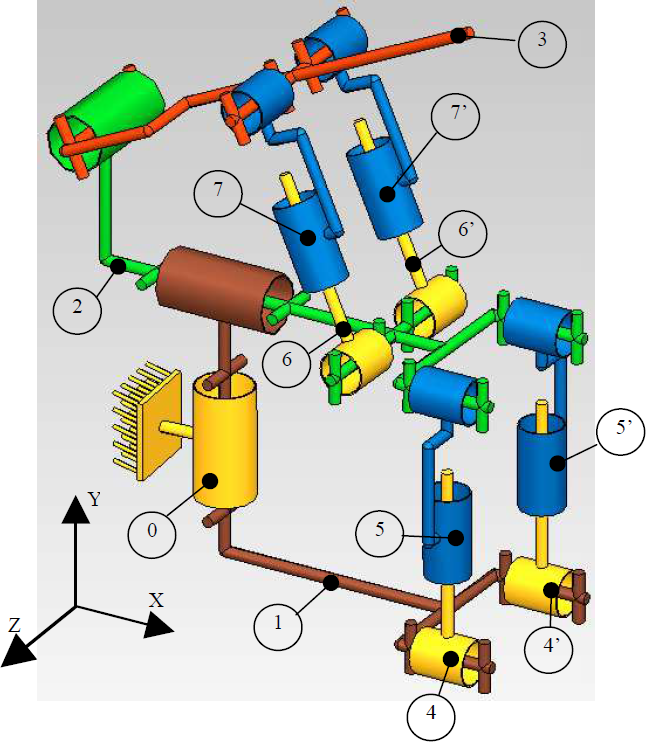
\includegraphics[width=\linewidth]{64_02}
\end{marginfigure}


\question{Déterminer le gain $K_c$ qui donne une marge de phase de 50\degres.}
\ifprof

Lorsque la phase vaut $-130\degres$, la gain vaut $-\SI{4}{dB}$. Il faut donc augmenter le gain de 4 dB soit $K_C = 10^{4/20} \simeq 1,6$. 

\begin{figure}[!h]
 \begin{tikzpicture}[xscale=2]
\tikzset{
semilog lines/.style={thin, bleuxp}, 
semilog lines 2/.style={semilog lines,bleuxpc},
semilog half lines/.style={semilog lines 2,dotted },
semilog label x/.style={semilog lines,below,font=\tiny,black},
semilog label y/.style={semilog lines,right,font=\tiny,black}
}
\begin{scope}[yscale=1/60]
\OrdBode{20}
\semilog{-1}{2}{-80}{40}

\BodeAmp[bleuxp,thick]{-1:2}{\POAmpAsymp{1}{3.6}+\IntAmp{4}}
\BodeAmp[orangexp,ultra thick]{-1:2}{\POAmp{1}{3.6}+\IntAmp{4}}
%\draw (-2.2,27) node {\footnotesize 23,5 dB, 0 dB/d\'ecade};
%\draw (-3.5,120) node {\footnotesize $-$20 dB/d\'ecade};
%\draw (-1.5,65) node {\footnotesize $-$40 dB/d\'ecade};
%\draw [dashed,ultra thick,bleuxp] (-2.47,-1) -- (-2.47,80);
%\draw (-2.47,-1)  node {\Huge $\cdot$} node [above right]{\footnotesize $\dfrac{1}{300}$};
\end{scope}
\begin{scope}[yshift=-2cm,yscale=1/150]
\UniteDegre
\OrdBode{45}
\semilog{-1}{2}{-270}{0}
%\BodeArg[orangexp,samples=200,thick]{-1:1}{\POArgAsymp{40.}{300.}+\IntArg{1}}
\BodeArg[bleuxp,thick]{-1:2}{\POArgAsymp{4}{3.6}+\IntArg{1}}
\BodeArg[orangexp,ultra thick]{-1:2}{\POArg{4}{3.6}+\IntArg{1}+\RetArg{.2}}
\end{scope}
\end{tikzpicture}
\end{figure}


\else 
\fi

\question{La constante $T_c$ qui laisse subsister une marge de phase d’environ 45\degres.}
\ifprof
Le gain est nul pour une pulsation de $\SI{1,5}{rad/s}$ On veut que $T_c$ n'affecte pas la marge de gain. On place donc $T_c$ une décade plus tôt, c'est à dire tel que $1/T_c = 1,5/10$ soit $T_c = \SI{6,7}{s}.$ 
\else 
\fi


\question{Quelle est l’erreur de traînage du système corrigé pour l’entrée en rampe considérée (en négligeant le retard).}
\ifprof
\else 
\fi


\ifprof
\else



\marginnote{Corrigé voir \ref{PERF:02:C2:03:stab:64}.}

\fi